\section{Side by side comparison}
\label{sec:comparison}

In this section we compare both results side by side. Firstly, the output of the envelope detector (take note that the theoritcal analysis one is the plot in orange):
\begin{figure}[h]
    \centering
    \begin{subfigure}{0.23\textwidth}
        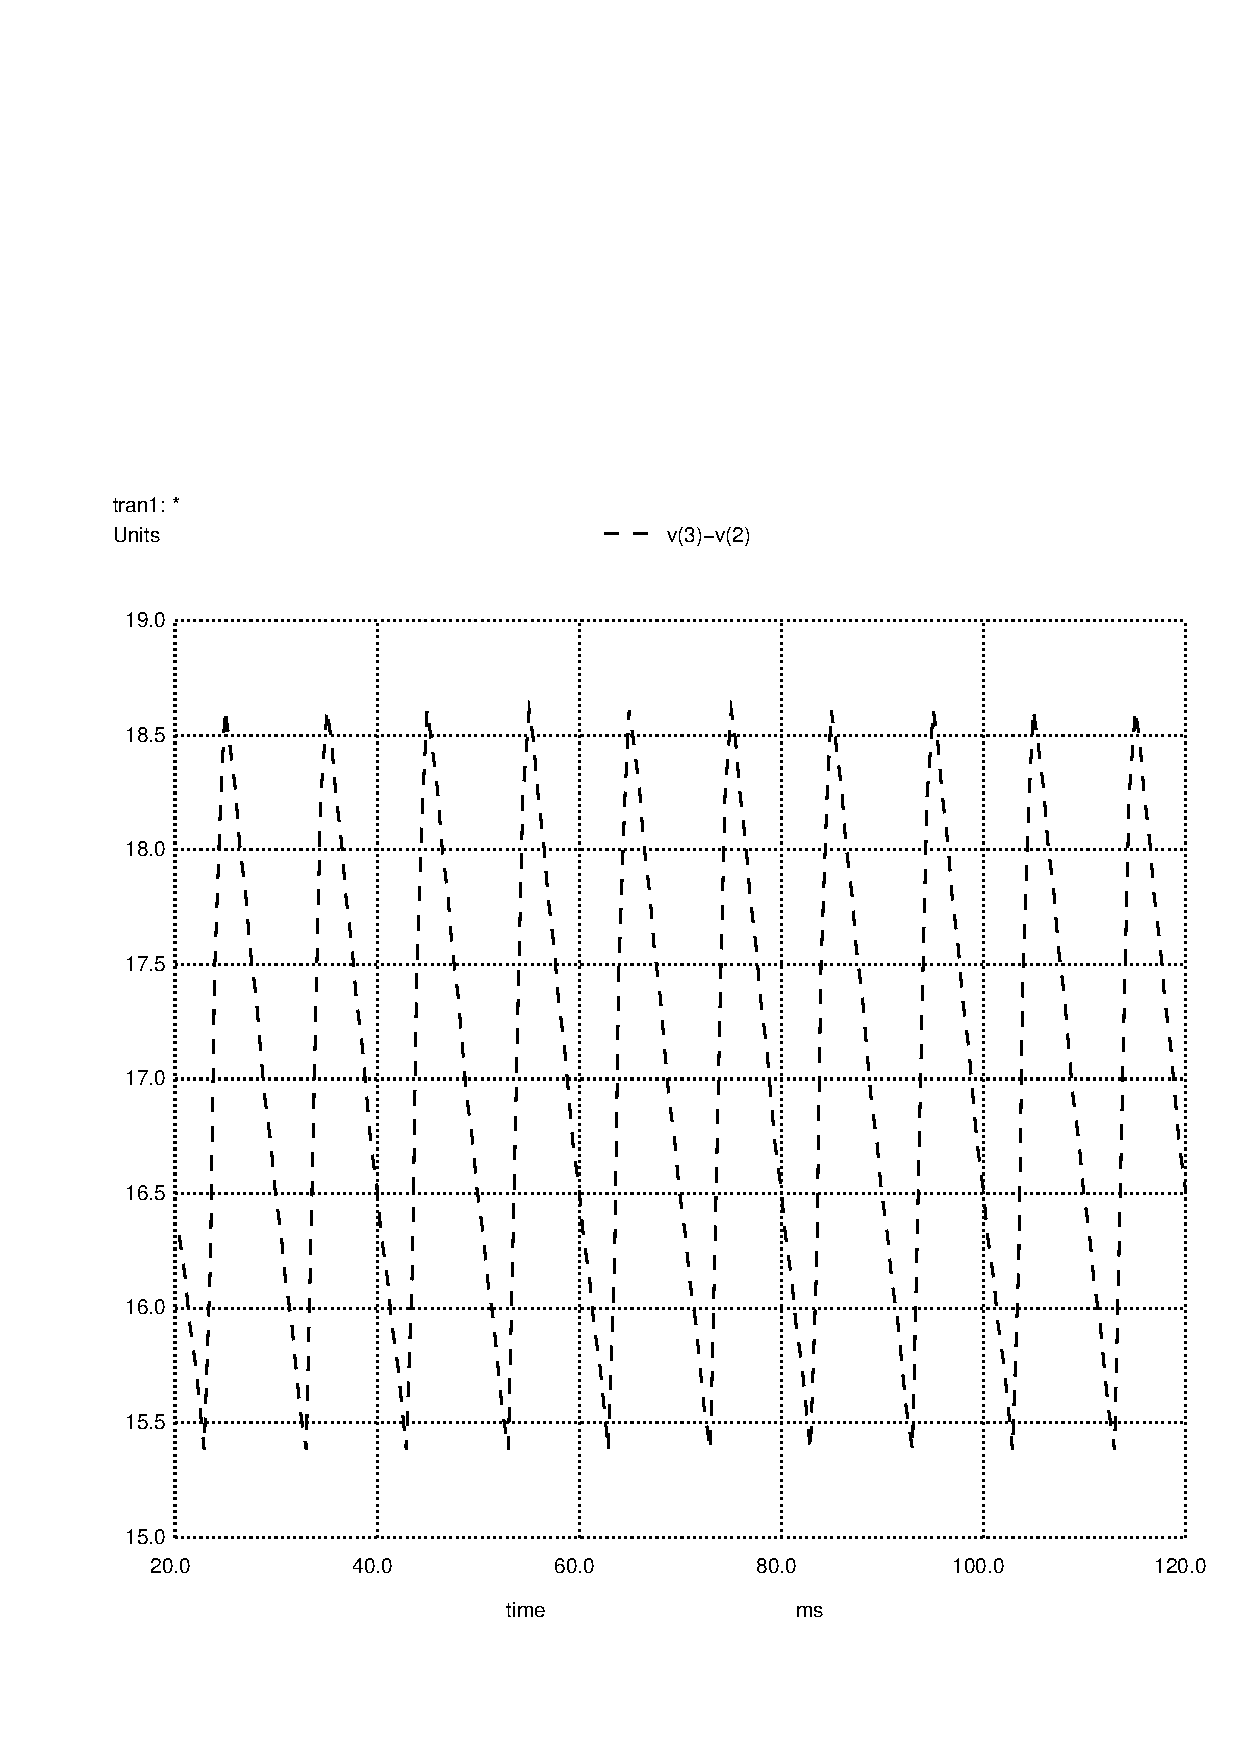
\includegraphics[width=\linewidth, clip]{solution2.pdf}
        \label{fig:envd1}
    \end{subfigure}
    \begin{subfigure}{0.23\textwidth}
        \includegraphics[width=\linewidth, clip]{venvlope.eps}
        \label{fig:envd2}
    \end{subfigure}
    \caption{\small Envelope detector output (left - simulation; right - theoretical )}
    \label{env_detector}
\end{figure}

\begin{figure}[h]
    \centering
    \begin{subfigure}{0.23\textwidth}
        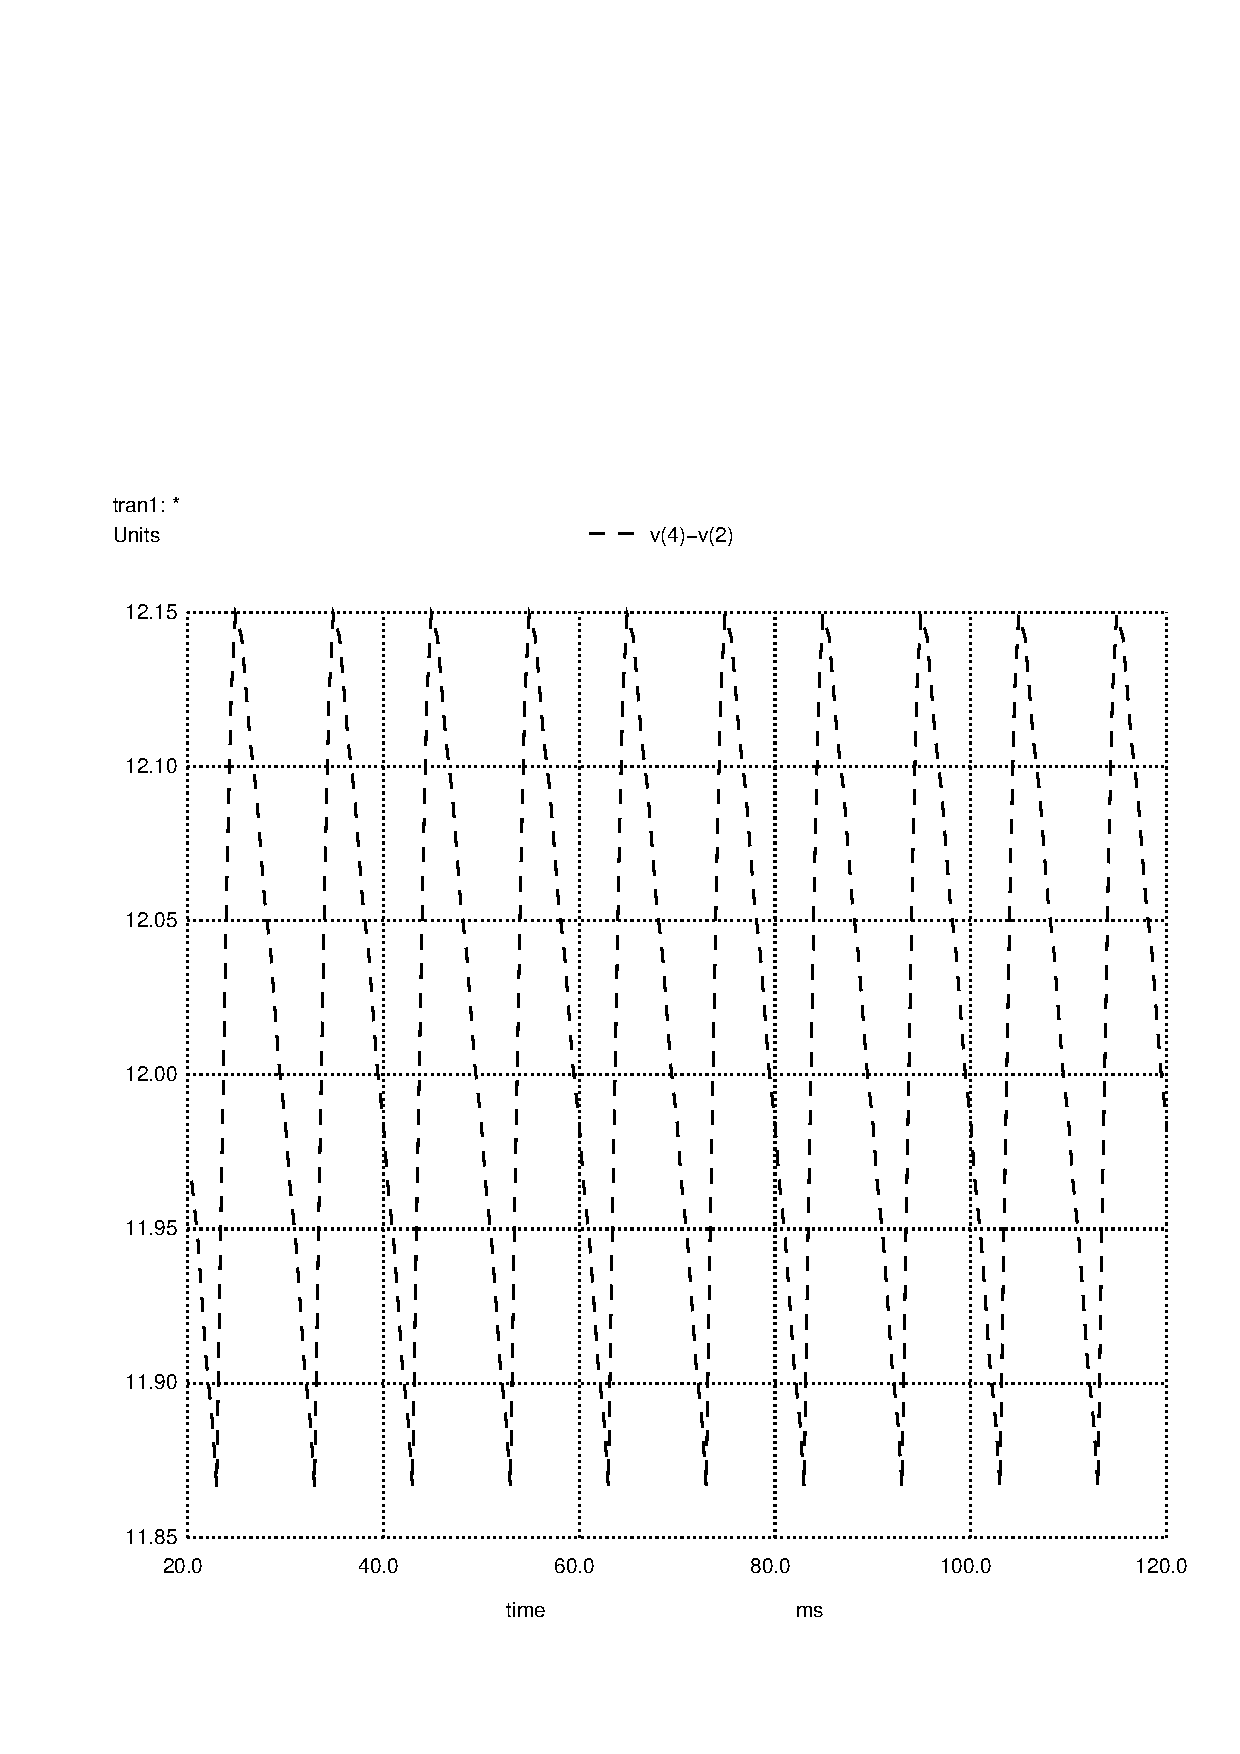
\includegraphics[width=\linewidth, clip]{solution1.pdf}
        \label{fig:voltr1}
    \end{subfigure}
    \begin{subfigure}{0.23\textwidth}
        \includegraphics[width=\linewidth, clip]{voltageRegulator.eps}
        \label{fig:voltr2}
    \end{subfigure}
    \caption{\small Voltage regulator output (left - simulation; right - theoretical )}
    \label{volt_reg}
\end{figure}

The shape of the graphs, both envelope detector and voltage regulator is similar, so we can concluse that both fullfill their purposes and the theoretical model used was good at predicting the general behaviour of the circuit. 
However, especially on the voltage regulator graphs, we can see some differences in the scale of the oscillations, that can be due to the different models used in our theoretical simulation, compared to ngspice.
We will quantify this difference later in the difference of the ripple in both simulations.

\begin{figure}[h]
    \centering
    \begin{subfigure}{0.23\textwidth}
        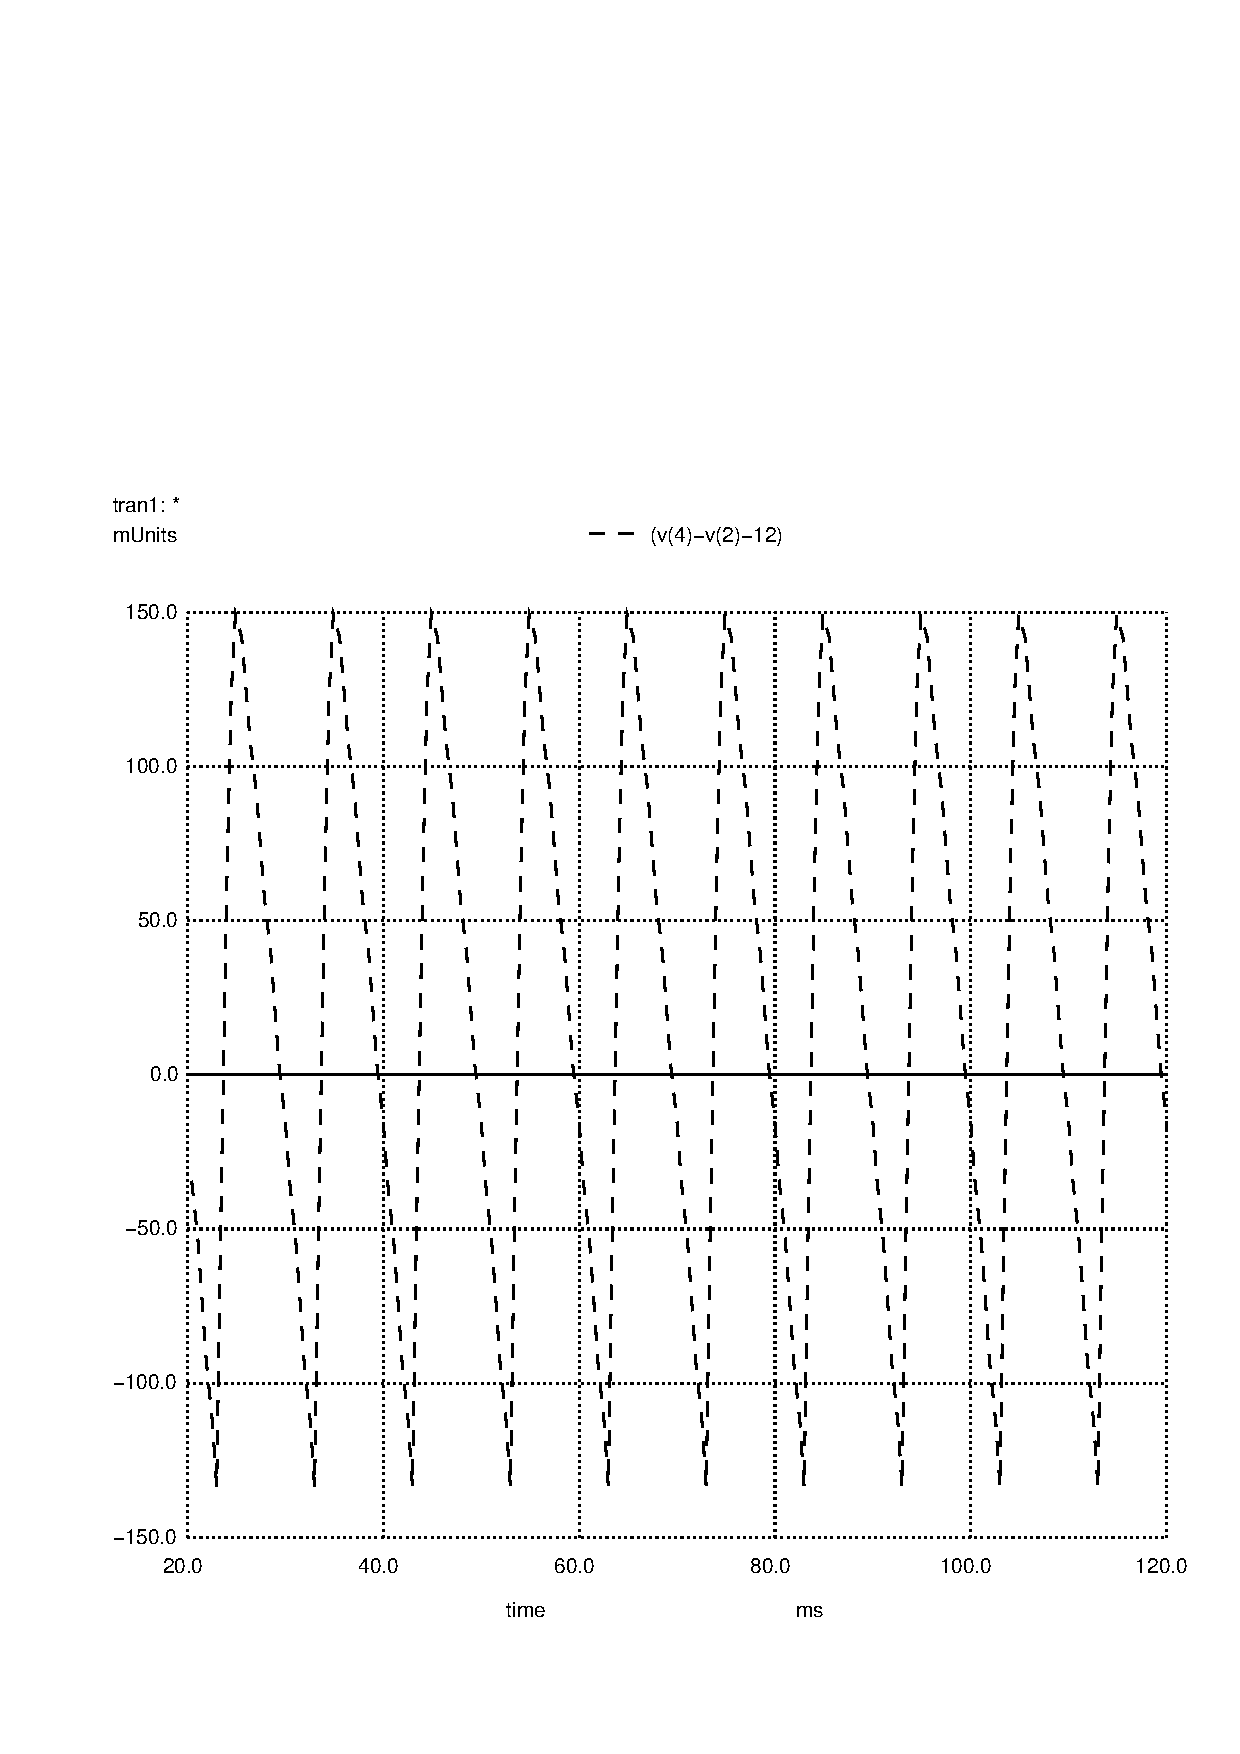
\includegraphics[width=\linewidth, clip]{solution12.pdf}
        \label{fig:output1}
    \end{subfigure}
    \begin{subfigure}{0.23\textwidth}
        \includegraphics[width=\linewidth, clip]{Deviation.eps}
        \label{fig:output2}
    \end{subfigure}
    \caption{\small $V_Out - 12$ - measure of the output DC deviation + AC component (left - simulation; right - theoretical )}
    \label{output_deviation}
\end{figure}

Once again, as in the previous graphs, the output deviation graph has a similar shape but a noticeable difference in scale, probably due to different models.



\section{Conclusion}
\label{sec:conclusion}


The ultimate goal of this laboratory assignment, to analyse
the given circuit theoretically and using simulation (and consequently
familiarising the group with the tools used), has been achieved, since
the simulation results matched the theoretical results with great accuracy.
These results were expected because we use the same linear models to
describe the behaviour of the components in \textit{Ngspice} and in
theoretical analysis (\ref{sec:analysis}). Furthermore, none of
the components is time dependent.

%\lipsum[1-1]
